% Asset ID: AS1VectorsTikZ-001
% Asset type: TikZ diagram
% Suggested file: tikz/AS1VectorsTikZ-001_vector_components.tex
% Source: CCEA AS1-VEC-LO001, AS1-VEC-LO002; Phase 1 Core Theory
% Related lesson section: Key Definitions and Notation; Core Theory 1 and 2
% Purpose: Show a 2D vector split into horizontal i and vertical j components.
% Boundary note: 2D vectors only. No k notation or 3D vectors.

\documentclass[tikz,border=8pt]{standalone}
\usepackage{amsmath}
\usetikzlibrary{arrows.meta, positioning}
\begin{document}
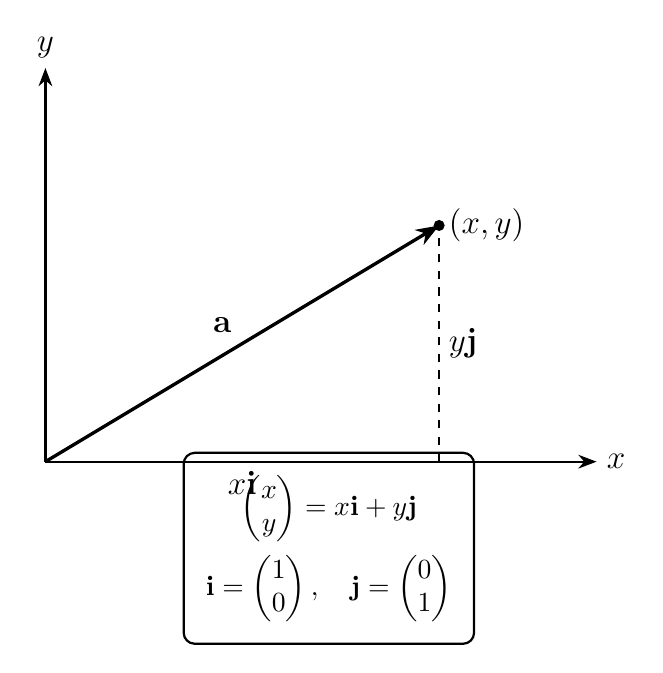
\begin{tikzpicture}[>=Stealth,axis/.style={->, thick},vector/.style={->, very thick},guide/.style={dashed, thick},label/.style={font=\large},formula/.style={draw, rounded corners, thick, align=center, inner sep=8pt}]
\draw[axis] (0,0) -- (7,0) node[right,label] {$x$};
\draw[axis] (0,0) -- (0,5) node[above,label] {$y$};
\coordinate (O) at (0,0); \coordinate (P) at (5,3);
\draw[guide] (O) -- (5,0); \draw[guide] (5,0) -- (P);
\draw[vector] (O) -- (P) node[midway, above left,label] {$\mathbf{a}$};
\fill (P) circle (2pt); \node[label,right] at (P) {$(x,y)$};
\node[label,below] at (2.5,0) {$x\mathbf{i}$}; \node[label,right] at (5,1.5) {$y\mathbf{j}$};
\node[formula] at (3.6,-1.1) {$\displaystyle \begin{pmatrix}x\\y\end{pmatrix}=x\mathbf{i}+y\mathbf{j}$\\[4pt] $\displaystyle \mathbf{i}=\begin{pmatrix}1\\0\end{pmatrix},\quad \mathbf{j}=\begin{pmatrix}0\\1\end{pmatrix}$};
\end{tikzpicture}
\end{document}
